\section{Introduction}

Clear demonstration that the proton has a finite size (unlike the electron?) had to wait for the availability 
of electron beams with energy up to 500 MeV. In his extensive, 1956, review Robert Hofstadter presented data
for the angular distribution of the elastically scattered electrons up to 140 degrees which differ from the
expectation for a point charge and magnetic distribution by a factor of 5 at the largest
$ q^2= 10^{-24}cm^2$ or 0.65 GeV$^2$. A proton radius of 0.80 fm was derived from these data.
We take note that the JLab data from  double polarization experiments completed in 2000 with electrons of
5 GeV differed from what was then believed to be the gold standard proton form factors by a similar
factor; the standard data base at the time was entirely defined by cross section measurements, and
suggested that both the electric and magnetic form factors behaved approximately like the dipole form
factor $G_D=(1+\frac{Q^2}{0.71})^{-2}$, with the momentum transfer squared Q$^2$ is in units of GeV$^2$.
The series of experiments started in 1998 in Hall A at JLab showed that the electric and magnetic form
factor ratio decreased linearly with Q$^2$, reaching a factor 1/5 at the highest Q$^2$ investigated so
far (5.6 GeV$^2$). And almost 60 year after this work we are discussing whether the proton radius is
\~0.875 or 0.76 fm.

\subsection{Dirac and Pauli Form Factors}

The lowest order approximation for electron nucleon scattering is the single virtual photon exchange model,
 or Born term. The approximation is expected to be valid because of the weak electro-magnetic coupling of
 the photon with the charge and magnetic mooment of the nucleon. The amplitude for the process is the
product of the four-component leptonic and hadronic currents, $\ell_{\nu}$ and ${\mathcal J}_{\mu}$,
can then be written as:
\begin{eqnarray}
i{\mathcal M}=\frac{-i}{q_{\mu}^2}\ell_{\mu}{\mathcal J}^{\mu}\frac{-ig_{\mu\nu}}{q_{\mu}^2} \nonumber \\
             \times\left[ie\bar{u}(k')\gamma^{\nu}u(k)\right]\left[ie\bar{v}(p')\Gamma^{\mu}(p',p)v(p)\right]
\end{eqnarray}
where $\Gamma^{\mu}$ contains all information of the nucleon structure, and $g_{\mu\nu}$
is the metric tensor. To insure relativistic invariance of the amplitude
$\mathcal M$, $\Gamma^{\mu}$ can only contain p, p' and $\gamma^{\mu}$, besides numbers,
masses and Q$^2$.

The most general form for the hadronic current for the spin $\frac{1}{2}$-nucleon, satisfying relativistic invariance
and current conservation and including an internal structure is:\\
\begin{equation}
{\mathcal J}_{hadronic}^{\mu}=ie\overline{\nu}(p')\left[\gamma^{\mu}{{F_1(Q^2)}}+
\frac{i\sigma^{\mu\nu}q_{\nu}}{2M_p}\kappa_{j}{{F_2(Q^2)}}\right]\nu(p), \\
\label{eq:Jhadron}
\end{equation}
\noindent where j=p,n and $Q^2=\vec{q}^{~2}-\omega^2=-q_{\mu}^{ 2}$, is the negative of the square of the
invariant mass $q_{\mu}^2 $ of the virtual photon exchanged in the one-photon
approximation of $e{\it N}$ scattering. $F_1(Q^2)$ and $F_2(Q^2)$, the Dirac and Pauli form factors, are the only ones
allowed in the Born term by relativistic invariance. $\kappa_p=\mu_p-1$ and $\kappa_n=\mu_n$ the anomalous
 magnetic moments of the proton
 and neutron, respectively, in units of the nuclear magneton, $\mu_N=\frac{e\hbar}{2M}$. The values of
$\kappa_p=$1.7928 and $\kappa_n$=-1.9130, with  ${M}$ the nucleon mass.
In the static limit, $Q^2=0$, $F_{1p}=1$, $F_{2p}=\kappa_p$ and $F_{1n}=0$ and $F_{2n}=\kappa_n$,
for the proton and neutron, respectively.

The Lab frame differential cross section for detection of the electron in elastic $ep$ or $en$ scattering is then:
\begin{eqnarray}
\frac{d\sigma}{d\Omega_e}&=&\left(\frac{d\sigma}{d\Omega}\right)_{Mott} \nonumber \\
 &\times&\left[F_1^2(Q^2)+\tau \left\{F_2^2(Q^2)+2(F_1(Q^2)+F_2(Q^2))^2\tan^2\frac{\theta_e}{2}\right\}\right]
\end{eqnarray}
\noindent
where with $\tau=Q^2/4M_p^2$ and $(\frac{d\sigma}{d\Omega})_{Mott}$ is the Mott cross section, including the recoil factor
$\frac{E_e}{E_{beam}}=(1+\frac{2E_{beam}}{m}\sin^2\frac{\theta_e}{2})^{-1}$, given by:
\begin{equation}
\left(\frac{d\sigma}{d\Omega}\right)_{Mott}=\frac{\alpha^2}{4E_{beam}^2\sin^4
\frac{\theta}{2}}\frac{E_e}{E_{beam}}\cos^2\frac{\theta}{2}
\label{eq:csF1F2}
\end{equation}

Experimental cross section data are most easily analyzed in terms of another set of form factors, the Sachs form
factors $G_{Ep}, G_{En}$ and $G_{Mp}, G_{Mn}$:

\begin{eqnarray}
G_{E_{p,n}}& = & F_{1_{p,n}}-\tau F_{2_{p,n}}\\
G_{M_{p,n}}& = & F_{1_{p,n}}+F_{2_{p,n}},
\label{eq:gepgmp}
\end {eqnarray}
\noindent
 The scattering cross section Eq.~\ref{eq:csF1F2}
can then be written in a much simpler form, without interference term, leading to a
separation method for $G_{E_{p}}^2$ and $G_{M_{p}}^2$ known as Rosenbluth (or Longitudinal-Transverse) method,
as will be seen below. Now the cross section is:
\begin{equation}
\frac{d\sigma}{d\Omega}=\left(\frac{\alpha}{2E\sin(\frac{\theta_e}{2})\right}\right)^2\frac{E_e}{E_{beam}} \nonumber \\
                       \times&\left(\frac{\cot^2(\frac{\theta_e}{2})}{1+\tau}\left[G_{E_{p}}^2+\tau{G_{M_{p}}}^2\right] + 2\tau{G_{M_{p}}}^2\right)
\label{eq:csF1F2}
\end{equation}
\noindent
where $r_e$ is the electron Compton wave length. $G_{E_{p}}$, $G_{M_{p}}$, $G_{E_{n}}$
and $G_{M_{n}}$ have the static values of the charge and magnetic moments, of the proton
and neutron, respectively:
\begin{eqnarray}
G_{E_{p}}&=&1, \mbox{   }G_{M_{p}}=\mu_p; \mbox{    }F_{1_{p}}=1,\mbox{   }F_{2_{p}}=1\\
G_{E_{n}}&=&0, \mbox{   }G_{M_{n}}=\mu_n; \mbox{    }F_{1_{n}}=0,\mbox{   }F_{2_{n}}=1.\\  
\end{eqnarray}

Defining the polarization of the virtual photon as $\epsilon G_E^2+\tau G_M^2$ leads to the simpler form for
 the cross section: $\epsilon=\frac{1}{1+2(1+\tau))\tan^2\frac{\theta_e}{2}$, equ. \ref{eq:csF1F2} takes the much simpler form:

\begin{equation}
\frac{d\sigma}{d\Omega} = (\frac{d\sigma}{d\Omega})_{Mott}\left[G_E^2+\frac{\tau}{\epsilon}G_M^2\right]/(1+\tau)
\label{eq:csGEGM}
\end{equation}

%\begin{figure}[h!]
%\resizebox{0.4\textwidth}{!}{%
%  \includegraphics {FIG2.eps}
%}
%\caption{whatever}
%\label{fig:geplt2}
%\end{figure}

The modern version of the Rosenbluth separation technique takes advantage 
of the linear dependence in $\epsilon$, of the FFs in the reduced 
cross section based on Eq. (\ref{eq:csGEGM}), as follows:
\begin{equation}
\left(\frac{d\sigma}{d\Omega}\right)_{reduced} &=& \frac{\epsilon(1+\tau)}{\tau}\left(\frac{d\sigma}{d\Omega}\right)_{exp}/ \left(\frac{d\sigma}{d\Omega}\right)_{Mott} \nonumber \\
                                              &=& G_{M}^2+\frac{\epsilon}{\tau}G_{E}^2,
\label{eq:redcs}
\end{equation}
\noindent 
